\chapter{特征融合及RLCCD框架验证}
\label{chap:fusion}
本章主要对面向代码克隆检测的多维源代码表征方法整体框架RLCCD进行介绍,同时进行实验评估及验证。具体地,RLCCD是由上述基于预训练辅助模型的Token表征学习、基于子树划分的抽象语法树表征学习、基于图过滤的程序依赖图表征学习方法三种维度融合形成并进行实现的表征方法,最后通过与SourcererCC、ASTNN、SCDetector进行对比实验以验证该框架的有效性。
\section{特征融合}
特征融合方法是指将不同来源或不同层次的特征进行组合,合并成一个比输入特征更具有判别能力的特征,该多维特征能够在低维空间中高效计算实体和关系的语义联系,提高特征的表达能力和分类效果,有利于下游代码克隆检测任务的学习。

因此,经过第\ref{chap:Token}、\ref{chap:AST}、\ref{chap:PDG}章的表征学习,得到三种维度的特征向量:属性特性$V^{Token}$、结构特征$V^{AST}$、语义特征$V^{PDG}$。上述三种表征方式得到的特征向量通常具有信息互补性,且不同维度的特征是代码表示的平行语料,具有信息等价性,因此,本文提出了基于多模态学习的特征融合方法,将三个维度的特征向量通过特征融合生成多维表示。然后将多维表示送入单层线性网络。本文设计了两个特征融合方式:特征连接(Feature concatenation)和特征加法(Feature addition),如下图\ref{fig:concat_add}所示。

\begin{figure}[H]
  \centering
  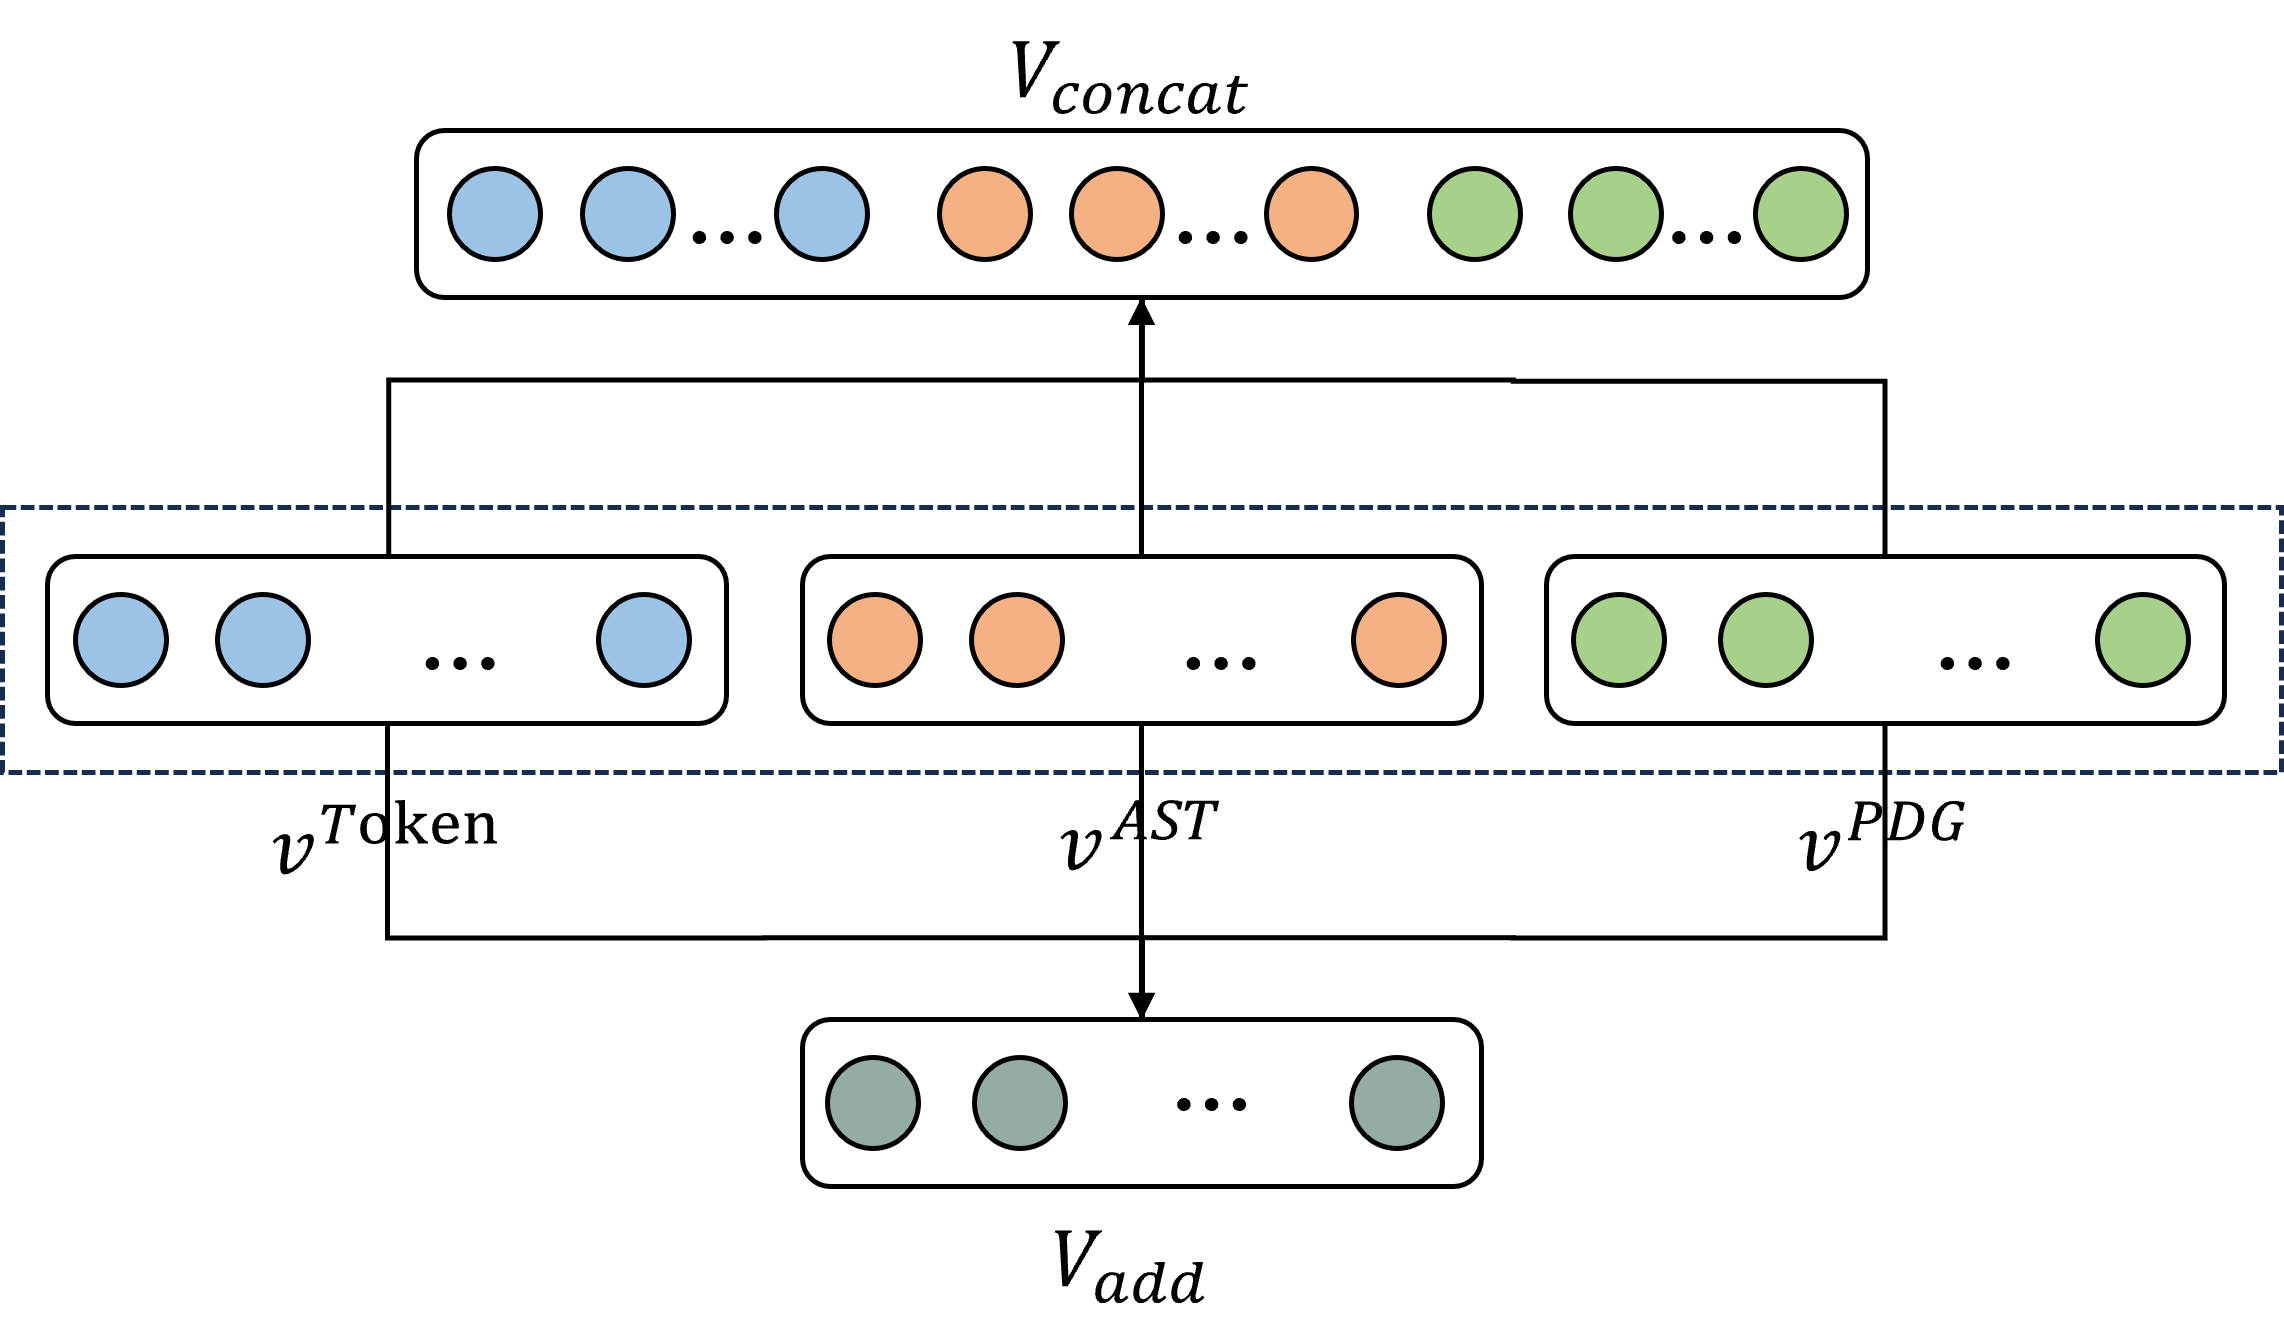
\includegraphics[width=0.55\textwidth]{figures/concat_add.png}
  \caption{特征融合方法}\label{fig:concat_add}
\end{figure}

其中特征连接是指直接将两个特征张量在某个维度上连接在一起,生成一个更大的张量。例如两个输入特征x和y的维数若为p和q,输出特征z的维数为p+q。在连接时,采取串联策略,两个张量的维度必须保持一致。而特征加法是指将两个特征张量按照元素相加在一起,生成一个新的张量。采取并行策略,特征向量本身的维度并没有增加。因此可以用公式\ref{e6.1}表示:

\begin{equation}\label{e6.1}
  \begin{split}
    \tilde{V_{concat}} &= concat \left( V^{\text{Token}} , V^{\text{AST}} , V^{\text{PDG}}\right) \\
    \tilde{V_{add}} &= add \left( V^{\text{Token}} , V^{\text{AST}} , V^{\text{PDG}}\right) \\
    V &= W_{dt} \cdot \tilde{V} + b_{dt}
  \end{split}
\end{equation}

其中$V$表示最终的多维混合代码表示,$W_{dt}$在生成的多维混合表示中平衡属性特征、结构特征、语义特征的组成,而$b_{dt}$在训练模型时使模型偏向最终收敛。

\section{RLCCD框架验证}
本文的实验设计主要围绕以下4个方面的研究问题:

• RQ1:本文提出的预训练辅助模型策略是否优于基线方法?(见3.3 节)

• RQ2:本文提出的子树划分策略是否优于基线方法?(见4.3 节)

• RQ3:本文提出的图过滤策略能否优于基线方法?(见5.3 节)

• RQ4:与现有代码克隆检测工具相比,RLCCD 表现如何?

\subsection{实验设置}
(1)系统环境

本章实验均在Ubuntu 16.04 LTS(64位)系统下进行。


(2)实验数据集

本章实验部分采用的数据集为代码克隆检测领域常见的基准集POJ104,该数据集是一个基于C语言构建的大型数据集,包含了104个编程问题以及学生提交的对应问题的不同C语言源代码,在该数据集中,针对同一问题的不同源解法的代码被视为一个克隆对。

\subsection{对比工具}
在对比整个方法的效果时,本文选取开源的SourcererCC、ASTNN、SCDetector方法进行比较。

SourcererCC:SourcererCC是一种相对较新的基于token的克隆检测工具。该工具通过词袋模型,把收集的数据全部编码成词频信息,后将代码行转换成一个由词频构成的向量,通过向量的比较获取相似度。

ASTNN:一种基于神经网络的源代码表示方法。它将整个抽象语法树AST分解成一系列小型语句子树,并通过捕获语句的词法和语法信息将语句子树分别编码为向量,最后采用了RNN模型生成代码片段的向量表示。ASTNN方法完整保留了抽象语法树的结构信息,能够检测到所有类型的代码克隆。

SCDetector:是基于令牌和基于图的方法的结合。给定一个方法源代码,我们首先生成CFG,然后应用中心性分析将图转换为某些语义标记(即具有图细节的标记)。最后,这些语义标记被馈送到Siamese网络中,以训练模型并使用它来检测代码克隆对。

\subsection{RLCCD性能评估实验结果}

对比实验:体现框架的有效性


\begin{table}
  \centering
  \caption{RLCCD实验结果} %\label{tab:category}
  \begin{tabular*}{0.9\textwidth}{@{\extracolsep{\fill}}cccc}
  \toprule
    对比			&P		&R		&F1 \\
  \midrule
    SourcererCC			&0.11	&0.43		&0.17 \\
    ASTNN			&0.87		&0.95		&0.91 \\
    SCDetector			&0.97	&0.81		&0.82 \\
    RLCDD			&0.xx		&0.xx		&0.xx \\
  \bottomrule
  \end{tabular*}
\end{table}

\section{本章小结}
本章节主要对RLCCD框架进行了实验验证,以验证RLCCD的XXX能力。



